\PassOptionsToPackage{utf8}{inputenc}
\documentclass{bioinfo}
\copyrightyear{2017} \pubyear{2017}

\access{Advance Access Publication Date: Day Month Year}
\appnotes{Original Article}

\begin{document}
\firstpage{1}

\subtitle{Genome Analysis}

\title[OneD]{OneD: increasing reproducibility of Hi-C Samples with
abnormal karyotypes}

\author[Vidal \textit{et~al}.]{Enrique Vidal\,$^{\text{\sfb 1,2}*}$,
François le Dily\,$^{\text{\sfb 1,2}}$, Javier Quilez\,$^{\text{\sfb
1,2}}$, Ralph Stadhouders\,$^{\text{\sfb 1,2}}$, Yasmina
Cuartero\,$^{\text{\sfb 1,2}}$, Thomas Graf\,$^{\text{\sfb 1,2}}$, Marc A.
Mart\'i Renom\,$^{\text{\sfb 1,2}}$, Miguel Beato\,$^{\text{\sfb 1,2}}$
and Guillaume J. Filion\,$^{\text{\sfb 1,2}}$}

\address{$^{\text{\sf 1}}$Gene Regulation, Stem Cells and Cancer Program,
Centre for Genomic Regulation (CRG), The Barcelona Institute of Science
and Technology (BIST), Barcelona, Spain \\
$^{\text{\sf 2}}$Universitat Pompeu Fabra (UPF), Barcelona, Spain}

\corresp{$^\ast$To whom correspondence should be addressed.}

\history{Received on XXXXX; revised on XXXXX; accepted on XXXXX}

\editor{Associate Editor: XXXXXXX}

\abstract{
  \textbf{Motivation:} The three-dimensional conformation of genomes is an
essential component of their biological activity. The advent of the Hi-C
technology enabled an unprecedented progress in our understanding of
genome structures. However, Hi-C is subject to systematic biases that can
compromise downstream analyses. Several strategies have been proposed to
remove those biases, but the issue of abnormal karyotypes received little
attention. Many experiments are performed in cancer cell lines, which
typically harbor large-scale copy number variations that create visible
defects on the raw Hi-C maps. The consequences of these widespread
artifacts on the normalized maps are mostly unexplored. \\
	\textbf{Results:}
We observed that current normalization methods are not robust to the
presence of large-scale copy number variations, potentially obscuring
biological variations and enhancing batch effects. To address this issue,
we developed an alternative approach designed to take into account
chromosomal abnormalities. The method, called \textit{OneD}, increases
reproducibility among replicates of Hi-C samples with abnormal karyotype,
thus significantly outperforming previous methods.  In the absence of
chromosomal aberrations, \textit{OneD} fared equally well as
state-of-the-art methods, making it a safe choice for Hi-C normalization.
\textit{OneD} is fast and scales well in terms of computing resources for
resolutions up to 1 kbp. \\
\textbf{Availability:} \textit{OneD} is implemented as an R package
available at \href{http://www.github.com/qenvio/dryhic}
{http://www.github.com/qenvio/dryhic}. \\
\textbf{Contact:} \href{enrique.vidal@crg.eu}{enrique.vidal@crg.eu}\\	
\textbf{Supplementary information:} Supplementary data are available at
\textit{Bioinformatics}	online.}



\maketitle





%% --------------- Introduction --------------- %%

\section{Introduction}

One of the crown achievements of modern biology was to realize that
genomes have an underlying three-dimensional structure contributing to
their activity \citep{rowley2016three}. In mammals, this organization
plays a key role in guiding enhancer-promoter contacts
\citep{de2013topology}, in V(D)J recombination \citep{choi2014ctcf} and in
X chromosome inactivation \citep{galupa2015x}.

One of the most significant breakthroughs towards this insight was the
development of the high throughput chromosomal conformation capture
technology (Hi-C), assaying chromosomal contacts at a genome-wide scale
\citep{lieberman2009comprehensive}. Nowadays, exploring the spatial
organization of chromatin has become a priority in many fields and Hi-C
has become part of the standard molecular biology toolbox
\citep{denker2016second}.

Contrary to the precursor technologies 3C, 4C and 5C \citep{de2012decade},
Hi-C interrogates all possible pairwise interactions between restriction
fragments. However, this does not guarantee that the method has no bias.
On the contrary, local genome features such as the G+C content, the
availability of restriction enzyme sites and the mappability of the
sequencing reads have been shown to impact the results
\citep{yaffe2011probabilistic}. In addition, general experimental biases
such as batch effects. It is thus important to normalize Hi-C data in
order to remove biases and artifacts, so that they are not confused with
biological signal.

Several methods have been proposed to remove biases in Hi-C experiments
\citep{schmitt2016genome}. The first strategy is to model biases
explicitly from a defined set of local genomic features, such as the G+C
content. This approach is used in the method of
\cite{yaffe2011probabilistic} and in Hicnorm by \cite{hu2012hicnorm}. The
second strategy is to implicitly correct unknown biases by enforcing some
regularity condition on the data. This approach is used in the
Iterative Correction and Eigenvector decomposition method (\textit{ICE})
of \cite{imakaev2012iterative}, whereby the total amount of contacts of
every bin is imposed to be the same. \textit{ICE} is currently the most
popular method, due in part to its speed.

Neither of these strategies were designed with regard for cell types with
karyotypic aberrations, most common in cancer cells. Hi-C is very
sensitive to aneuploidy, copy number variations and translocations.
Actually, these aberrations have so much influence on the outcome that the
artifacts can be used to re-assemble the target genome
\citep{korbel2013genome}. So far the only attempt to address the issue
was the chromosome-adjusted Iterative Correction Bias method
(\textit{caICB}) of \cite{wu2016computational}.  However, caICB applies a
uniform chromosome-wide correction, effectively excluding the numerous
cases of partial aneuploidy and regional copy number variations.

Here we propose \textit{OneD}, a method to correct local chromosomal
abnormalities in Hi-C experiments. \textit{OneD} explicitly models the
contribution of known biases via a generalized additive model. The
normalized data is more reproducible between replicates and across
different protocols. Importantly, \textit{OneD} is also efficient when
cells have a normal karyotype, where it performs as well as the best
normalization methods. Finally, the implementation is as fast as
\textit{ICE} and it scales up to 1~kbp resolution with reasonable
computing resources.

%\enlargethispage{12pt}

\begin{methods}

\section{Methods}

\subsection{Model}
\label{sec:model}

The most common representation of Hi-C data is a contact matrix, obtained
by slicing the genome in $n$ consecutive bins of fixed size (the
resolution) and computing the number of contacts between each pair of
bins. The values are stored in the cells of the contact matrix ($x_{ij}$),
quantifying of the interaction between the tow loci at positions $i$ and
$j$.

Our approach is to model the tally of contacts for each bin, thus reducing
the matrix to a one dimension score (hence the name \textit{OneD}). We assume that
the total number of contacts per bin ($t_{i}$) can be approximated by a
negative binomial distribution. This choice is sensible because the amount
of contacts is a discrete variable and because the negative binomial
distribution allows for overdispersion. We further assume that the
explicit sources of bias have independent contributions to the mean of the
distribution for a given bin ($\lambda_i$).

Given that this relationship might not be linear (see for instance
Figure~\ref{fig:totals}A), we allowed a smooth representation
using thin plate penalized regression splines \citep{wood2003thin} in a
generalized additive model \citep{wood2011fast}. The model can be
parametrized as

\begin{align*}
t_i = \sum_j^n{x_{ij}} &\sim  NB(\lambda_i, \theta) \\
\log(\lambda_i) &\propto \sum_{k}{f_k(z_k)}
\end{align*}

\noindent
where $x_{ij}$ is the raw number of contacts between bins $i$ and $j$, and
$z_k$ is the additive bias of genomic feature $k$. The smooth functions
$\{f_k(\cdot)\}$ are estimated jointly with the negative binomial
dispersion parameter $\theta$ using the \texttt{mgcv} package
\citep{wood2011fast} of the R software \citep{coreteam2014r}.

Once the parameters of the model are estimated, we rescale the estimated
means $\{\lambda_i\}$ to obtain a correction vector $\{\lambda_i'\}$ that
can be used to compute the corrected counts ($\hat{x}_{ij}$).

\begin{align}
\notag
\lambda_i' &= \frac{\lambda_i}{\sum_j^n{\lambda_j}/n} \\
\label{eq:xhat}
\hat{x}_{ij} &= \frac{x_{ij}}{\sqrt{\lambda_i'\lambda_j'}}
\end{align}

In line with previous methods
\citep{yaffe2011probabilistic,hu2012hicnorm}, the features
used to fit the model are the local G+C content, read mappability and the 
content and number of restriction sites. The model and the implementation
can be easily extended with any user-provided genomic feature.

\subsection{Copy number correction}

Briefly, a hidden Markov model with emissions distributed as a Student's
$t$ variable is fitted on the corrected total amount of contacts per bin.
The model consists of 7 states that correspond to 1, 2, 3, 4, 5, 6 and 8
copies of the target, for a total of 3 emission parameters (a single
scaling parameter, a single standard deviation and a single degree of
freedom for all the states) and 21 transition parameters. 

The model is fitted with the Baum-Welch algorithm \citep{baum1966} until
convergence, following the detail given by \cite{filion2010systematic}.
The Viterbi path is then computed and corresponds to the inferred copy
number of each bin ($c_i$).

A correction equal to the square root of the copy number is then applied
to the whole matrix. More specifically, each cell is updated to


\begin{equation}
\label{eq:cnvnorm}
\hat{x}_{ij}^* = \frac{\hat{x}_{ij}}{\sqrt{c_ic_j}}
\end{equation}

\subsection{Data sources}

To test the correction of biases, we gathered a set of
published \citep{ledily2014distinct, encode2012integrated, rao20143d,
stadhouders2017transcription, lin2012global, dixon2012topological} and
unpublished Hi-C data of different cell types and organisms. The details
can be found in Table \ref{tab:samples}.

We used several experiments comprising T47D breast cancer cell
lines (7 samples), K562 leukemia cell lines (4 samples), both with
aberrant karyotypes, and mouse primary B (6 samples ) and ES (7 samples)
cells, both with normal diploid karyotypes. The experiments were carried
out in different laboratories, following either the original Hi-C protocol
\citep{lieberman2009comprehensive} or the newer \textit{in situ} version
\citep{rao20143d}, and using different restriction enzymes (DpnII,
HindIII, MboI and NcoI).

We also used array-based copy-number segmentation of the two cell
lines obtained from COSMIC database \citep{forbes2010cosmic}.

\begin{table*}
\processtable{Hi-C data sets used in this study. Sample ID: Unique sample
identifier. Cell type: Type of cell. Application: Hi-C protocol. RE: Restriction
enzyme used for digestion. Sequencing core: Laboratory performing the experiment
(CRG: Centre for Genomic Regulation; UMass: University of Massachusetts; Baylor: Baylor College of Medicine;
UCSD: University of California San Diego; LICR: Ludwig Institue for Cancer Research). Set(s): Comparison set. Source: SRA, GEO
or ENCODE raw data identifier.
\label{tab:samples}}
{\begin{tabular}{ccccccc}
  \toprule
  \textbf{Sample ID} & \textbf{Cell type} & \textbf{Application} &
  \textbf{RE} & \textbf{Sequencing core} & \textbf{Set(s)} &
  \textbf{Source} \\
  \midrule
dc3a1e069\_51720e9cf & T47D & \textit{in situ} Hi-C &
  DpnII & CRG & T47D, K562 & NA \\
b1913e6c1\_51720e9cf & T47D & \textit{in situ} Hi-C &
  DpnII & CRG & T47D & NA \\
dc3a1e069\_ec92aa0bb & T47D & \textit{in situ} Hi-C &
  DpnII & CRG & T47D, K562 & NA \\
HindIII\_T0 & T47D & dilution Hi-C &
  HindIII & CRG & T47D & SRR1054341 \\
NcoI\_T0    & T47D & dilution Hi-C &
  NcoI      & CRG & T47D & SRR1054343 \\
ENCLB758KFU & T47D & dilution Hi-C &
  HindIII   & UMass & T47D & ENCLB758KFU \\
ENCLB183QHG & T47D & dilution Hi-C &
  HindIII   & UMass & T47D & ENCLB183QHG \\
HIC069  & K562 & \textit{in situ} Hi-C &
  MboI & Baylor & T47D, K562 &    SRR1658693 \\
HIC070  & K562 & \textit{in situ} Hi-C &
  MboI & Baylor & T47D, K562 &    SRR1658694 \\
HIC071  & K562 & \textit{in situ} Hi-C &
  MboI & Baylor & K562 & SRR1658695,SRR1658696 \\
HIC074  & K562 & \textit{in situ} Hi-C &
  MboI & Baylor & K562 & SRR1658701,SRR1658702 \\
b7fa2d8db\_bfac48760 & B-cell  & \textit{in situ} Hi-C &
  DpnII & CRG & mm10 & GSE96611 \\
fc3e8b36a\_7bf1bf374 & ES-cell & \textit{in situ} Hi-C &
  DpnII & CRG & mm10 & GSE96611 \\
b7fa2d8db\_7284b867a & B-cell  & \textit{in situ} Hi-C &
  DpnII & CRG & mm10 & GSE96611 \\
fc3e8b36a\_38bfd1b33 & ES-cell & \textit{in situ} Hi-C &
  DpnII & CRG & mm10 & GSE96611 \\
b7fa2d8db\_58e812fc2 & B-cell  & \textit{in situ} Hi-C &
  DpnII & CRG & mm10 & GSE96611 \\
fc3e8b36a\_c990a254e & ES-cell & \textit{in situ} Hi-C &
  DpnII & CRG & mm10 & GSE96611 \\
b7fa2d8db\_73f11d923 & B-cell  & \textit{in situ} Hi-C &
  DpnII & CRG & mm10 & GSE96611 \\
fc3e8b36a\_4bf044f18 & ES-cell & \textit{in situ} Hi-C &
  DpnII & CRG & mm10 & GSE96611 \\
GSM987817 & B-cell  & dilution Hi-C &
  HindIII & UCSD & mm10 & SRR543428-SRR543431 \\
GSM987818 & B-cell  & dilution Hi-C &
  HindIII & UCSD & mm10 & SRR543432-SRR543442 \\
GSM862720 & ES-cell & dilution Hi-C &
  HindIII & LICR & mm10 & SRR443883-SRR443885 \\
GSM862721 & ES-cell & dilution Hi-C &
  HindIII & LICR & mm10 & SRR400251-SRR400256 \\
GSM862722 & ES-cell & dilution Hi-C &
  NcoI    & LICR & mm10 & SRR443886-SRR443888 \\
  \botrule
\end{tabular}}{}
\end{table*}

%\subsection{Data processing}

All data were processed though a pipeline based on TADBit
\citep{serra2016structural}. Briefly, after controlling the quality of
fastq files, paired-end reads were mapped in the corresponding reference
genome (hg38 and mm10) taking into account the restriction enzyme site.
Non-informative contacts were removed applying the following TADBit
filters: self-circle, dangling-ends, error, extra dangling-end, duplicated
and random-breaks. For more details, see the methods section of
\cite{stadhouders2017transcription}. In addition, the pipeline is
available from the supplementary material published by
\cite{quilez2017managing}.

We developed the routines contained in the \texttt{dryhic} R package to
efficiently create sparse representations of contact matrices and further
apply \textit{vanilla}, \textit{ICE} and \textit{oneD} corrections.
\texttt{HiTC} \citep{servant2012hitc} and \texttt{HiCapp}
\citep{wu2016computational} were used to carry out the \textit{LGF} and
\textit{caICB} corrections respectively. All the results are based on a
resolution of 100 kbp, but we found no major differences for different
values (not shown).



\subsection{Comparison of Hi-C matrices}
\label{sec:comp}

There is no universally accepted standard to compare Hi-C matrices. The
simplest metric is the Spearman correlation applied to intra-chromosomal
contacts up to a given distance (5 Mb in what follows). The second option
is to measure the similarity of observed over expected contacts via the
Pearson correlation up to a given distance range. Compared to the first,
this metric gives more weight to changes occurring away from the diagonal.
The third option is to compute a correlation per distance stratum and then
obtain a stratum-adjusted correlation coefficient (SCC) as defined in
\cite{yang2017hicrep}. Finally, the last option, proposed by
\cite{yan2017hicspector} is to measure the Pearson correlation between the
last eigenvectors of the Laplacian of the Hi-C matrix. This approach
borrows the concepts of spectral clustering \citep{von2007tutorial} and
amounts to comparing high level features of the matrix.

We defined three data sets to measure experimental reproducibility after
normalization: The first contained the samples from T47D plus two samples
from K562, the second contained the samples from K562 plus two samples
from T47D, the third contained all the mouse samples (see Table
\ref{tab:samples} for details). Given a set of experiments and a metric,
we first computed all pairwise combinations between experiments and then
classified the comparisons according to the characteristics of each pair
(cell type, protocol, batch and treatment).

To measure the gain or loss of similarity upon normalization, we compared
raw matrices to obtain a baseline. The differences with this baseline were
estimated using a linear mixed model fitted with the \texttt{lmer}
function of the \texttt{lme4} R package \citep{bates2015lme4}, where the
fixed effect was the normalization method and the random effect was the
%chromosome. Receiver operating characteristic (ROC) curves were then
computed using \texttt{ROCR} package \citep{sing2005rocr}.


\end{methods}




%% --------------- Results --------------- %%

\section{Results}

\subsection{Experimental bias correction}

The principle of \textit{OneD} is to explicitly model Hi-C biases on a
single variable: the total amount of contacts for each bin of the matrix
(see \ref{sec:model} for detail). The reason for this choice is that the
total amount of contacts is approximately proportional to the local copy
number. For instance, a duplicated region in a diploid genome will show on
average a 50\% increase in the number of contacts. Discontinuities of the
amount of contacts thus correspond to changes of the copy number.

\begin{figure}
\centerline{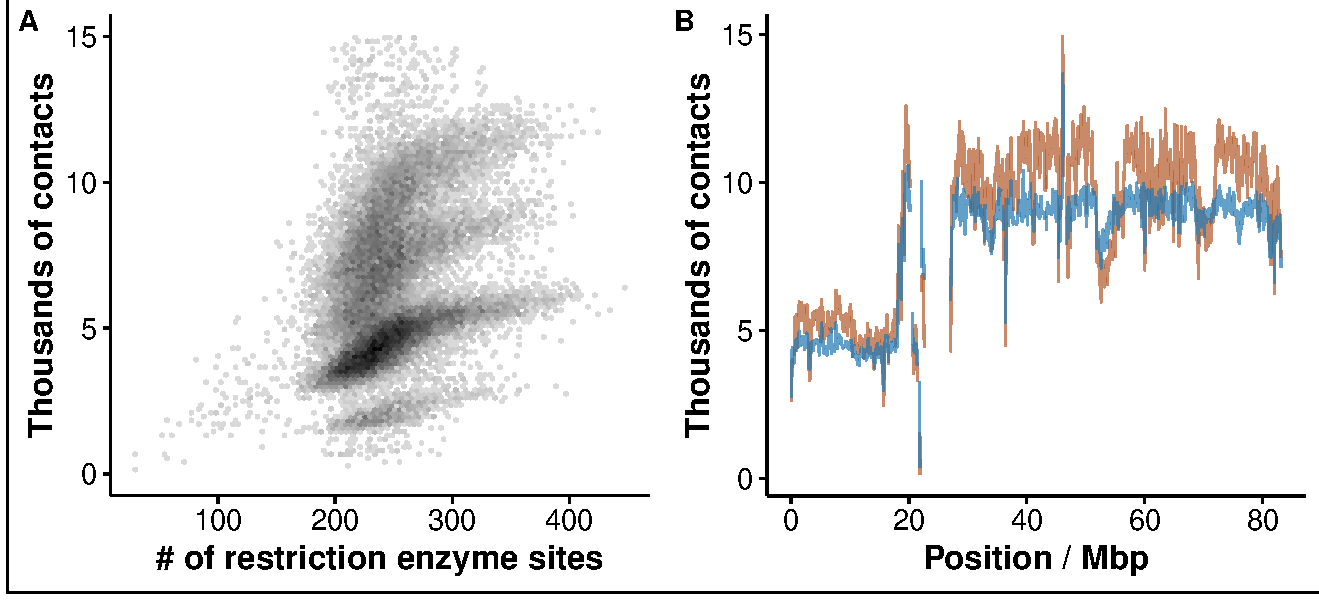
\includegraphics[width=.45\textwidth]{img/figure1.pdf}}
\caption{Total amount of contacts per bin. A. Non linear relationship
between the number of restriction sites and the total number of
contacts per bin in T47D. B. Total number of contacts per bin on
chromosome 17 of T47D. Raw (brown) and corrected (blue) signals are shown.
The long arm of chromosome 17 (the region corresponding to 20-40 Mbp) is
present in four coipes, explaining that the signal is about twice higher
than for the short arm.}
\label{fig:totals}
\end{figure}

Experimental biases affect the total amount of contacts in a continuous
but not necessarily linear way. Figure~\ref{fig:totals}A shows the
relationship between the amount of contacts and the number of restriction
enzyme sites in T47D, a breast cancer cell line with aberrant and unstable
karyotype.  Four clouds are visible. Each corresponds to sequences present
in one to four copies. In all of them, the relationship flattens as the
number of restriction sites increases. In order to capture this
relationship, \textit{OneD} fits a non-linear model between the total
amount of contacts and the known sources of bias (by default the G+C
content, the number of restriction sites and the mappability of the
reads).

The experimental biases are estimated genome-wide and each cell of the
matrix is then corrected using equation (\ref{eq:xhat}). Note that the
corrected amount of contacts is still proportional to the copy number.
Figure~\ref{fig:totals}B shows the corrected number of contacts along
chromosome 17 of T47D. \textit{OneD} greatly reduces the wiggling of the
total amount of contacts.

We tested the validity of this approach against the Catalogue Of Somatic
Mutations In Cancer \citep[COSMIC,][]{forbes2010cosmic}. In what follows,
we benchmarked \textit{OneD}, against \textit{vanilla}, \textit{ICE}
\citep{imakaev2012iterative}, \textit{caICB} \citep{wu2016computational}
and the Local Genomic Features method
\citep[\textit{LGF},][]{hu2012hicnorm, servant2012hitc}. The first three
methods correct biases implicitly, whereas the fourth method does it
explicitly. Figure \ref{fig:copy_number} shows the Pearson correlation
between the corrected number of contacts and the copy number estimation
for both T47D and K562 cell lines. Similar results were obtained using
Spearman correlation (Supplementary Figure 1). All the methods except
\textit{OneD} decrease the agreement between the signal and the copy
number because they partially correct the discrepancy. In contrast,
\textit{OneD} enhances the conformity of the signal with the copy number.
Not correcting for variable copy number at that stage may seem
counter-intuitive, but the tests below will show this leads to better
performance.


\begin{figure}[b]
	\centerline{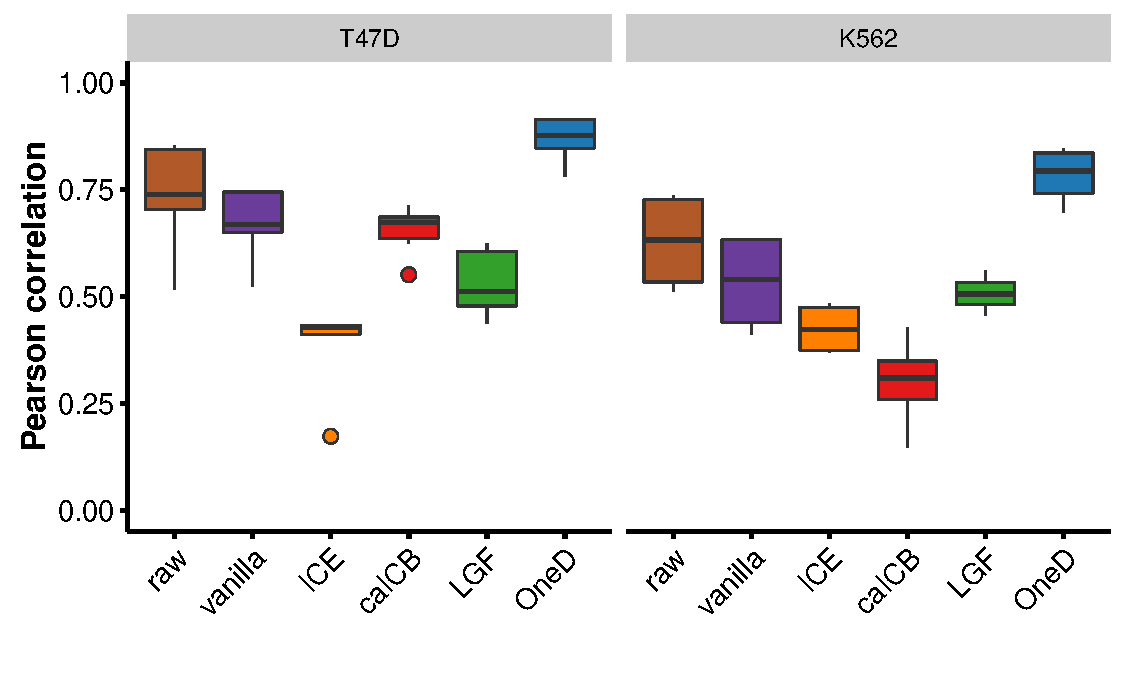
\includegraphics[width=.45\textwidth]
{img/copy_number_figure2.pdf}}
\caption{Pearson correlation between the total number of contacts per bin
and an independent estimation of the copy number (COSMIC). Left panel
T47D breast cancer cell line, right panel K562 leukemia cell line.}
\label{fig:copy_number}
\end{figure}




\subsection{Aberrant karyotypes}

We first benchmarked the performance of our approach on biological
samples with an aberrant karyotype. A good normalization method should
increase the similarity between biological replicates by reducing
irrelevant experimental variation, such as batch effects, laboratory of
origin and protocol variations. Similarly, a good normalization should
decrease the similarity between samples that received a different
treatment in order to enhance the biological differences.

We assembled two Hi-C data sets obtained from T47D and K562, two cancer
cell lines with aberrant karyotypes. In each set we spiked two samples
from the other cell line (see Table~\ref{tab:samples}) in order to
introduce biological variability. We compared matrices before and after
normalization by different methods using the Pearson correlation of
observed over expected counts (see \ref{sec:comp}). This gave an
indication of the impact of a given normalization method. The results are
summarized in Figure~\ref{fig:aberrant}.

The \textit{caICB} and \textit{ICE} methods increased the similarity
between the different cell lines (Figures~\ref{fig:aberrant}A and
\ref{fig:aberrant}B and Supplementary Figures~2 and 3). This is an undesirable
effect, as it obscures the biological variability. In the same vein, these
methods decreased the similarity between samples that received the same
treatment (Figure~\ref{fig:aberrant}A), suggesting that the normalization
process is detrimental to the biological signal in these two cases. The
method \textit{vanilla} followed the same trend but to a lesser extent,
consistent with the fact that it consists of a single \textit{ICE}
iteration. \textit{OneD} was the only method to increase the similarity
between experiments carried out on the same material but with a different
protocol (Figure~\ref{fig:aberrant}A).

An important application of normalization methods in experimental setups
is to identify outliers. We thus investigated the capacity of the
different methods to help identify the samples from the other cell type
spiked in the data set. We interpreted the pairwise comparison scores as
classifier scores and summarized the results with a ROC curve
(Figures~\ref{fig:aberrant}C and D).

All the methods, including the absence of normalization, succeeded in
identifying the T47D outliers among the K562 samples, but recognizing the
K562 outliers among the T47D samples proved more challenging.
\textit{OneD} increased the discrimination power compared to the raw
matrices, but all the other methods decreased it. Actually, they performed
little better than random on this task.

Using the other metrics described in \ref{sec:comp} yielded similar
results (Supplementary Figures 5, 6 and 7). Note that Spearman correlation
of contacts presented the worst performance for all scenarios, and it thus
seems to be a poor choice as a metric to compare HiC matrices.

Taken together, these results show that correcting experimental biases
with \textit{OneD} enhances the biological variation and reduces the noise
on samples with an aberrant karyotype.


\begin{figure}
\centerline{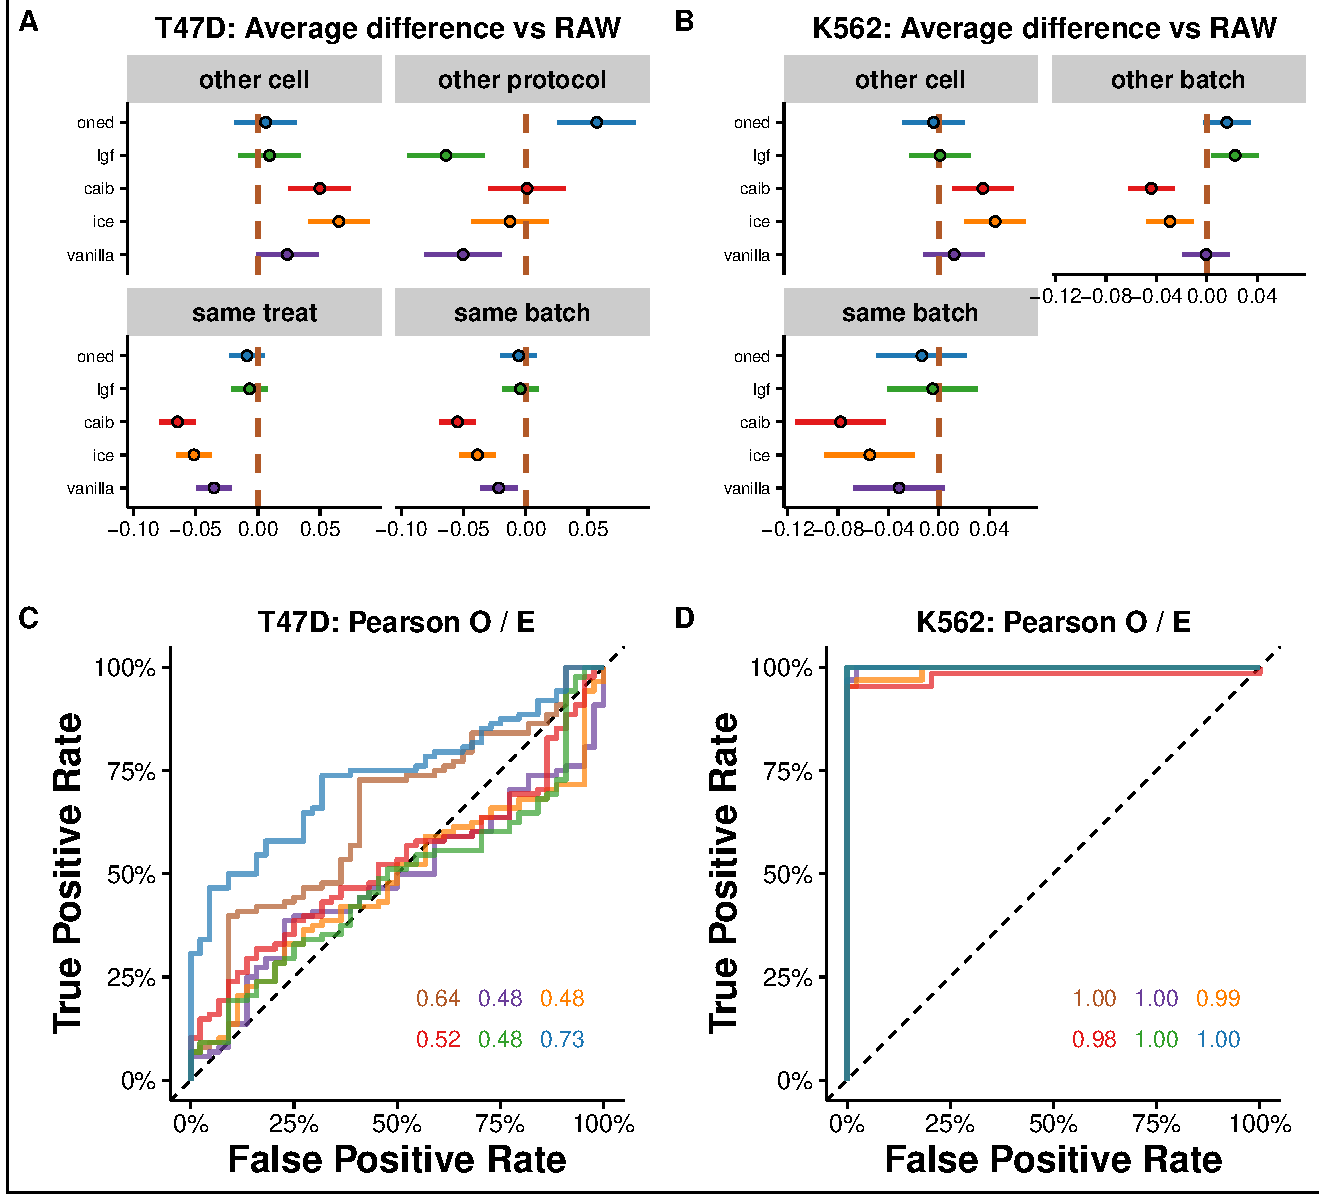
\includegraphics[width=.50\textwidth]
  {img/correlation_aberrant_figure3.pdf}}
\caption{
Results of the comparison between samples with aberrant karyotypes. A and
B. Average changes compared to the raw data on the T47D and K562 sets. The
bars represent 95\% confidence intervals centered on the mean difference
of the correlation score between a given correction method and the raw
data. C and D. ROC curves on the T47D and K562 sets.  The areas under the
curve are indicated in the bottom right corner. The color code is the same
as panels A and B. The brown lines correspond to raw matrices. All results
in this figure are based on Pearson correlations between the observed over
expected counts.}
\label{fig:aberrant}
\end{figure}



\subsection{Normal karyotypes}

Does the performance of \textit{OneD} for aberrant karyotypes come at the
cost of decreased performance for normal karyotypes? To address this
question, we assembled another data set comprised of mouse B cells and
embryonic stem (ES) cells, both with a normal karyotype The cell types
were pooled in almost equal proportions (see Table~\ref{tab:samples}) and
the same tests as above were performed.

In these conditions, the experimental protocol had a strong effect on the
impact of the different normalization methods (Figure~\ref{fig:normal}A).
For instance, \textit{caICB} and \textit{ICE} increased the similarity
when the protocols were different, but decreased it when the protocols
were the same. The effect was stronger when comparing identical cell
types, but the same trend appeared when comparing different cell types,
indicating that these methods may enhance or reduce biological variation,
depending on the context. Once more, \textit{vanilla} followed the same
trend as \textit{ICE} to a lesser extent. The \textit{LGF} method
increased the similarity when comparing the same cells with different
experimental protocols, and had little to no effect in the other cases.
This indicates that \textit{LGF} is a safe choice in this case.

\textit{OneD} decreased the similarity between different cell types when
using the same protocol and increased it between identical cell types when
using different protocols. In the other two cases, it had little effect.
In summary, \textit{OneD} never enhanced the experimental noise and it
reduced it in one more case than \textit{LGF}.

When interpreting the similarity scores as classification scores, we
observed that all the methods could identify approximately 50\% of the
biological pairs, after which their performance diverged
(Figure~\ref{fig:normal}B). \textit{OneD} achieved the highest area under
the curve on this problem, but with a small margin over the other methods
except \textit{vanilla}.

Using other metrics to compare matrices gave similar results
(Supplementary Figures 7 and 8). \textit{OneD} was always among the top
scoring methods. In these conditions, Spearman correlation of contacts
again appeared as the worst comparison metric because it showed a lower
performance for all the normalization methods.

Taken together, these results indicate that \textit{OneD} performs as well
as the best normalization methods, even with normal karyotypes.

\begin{figure}
\centerline{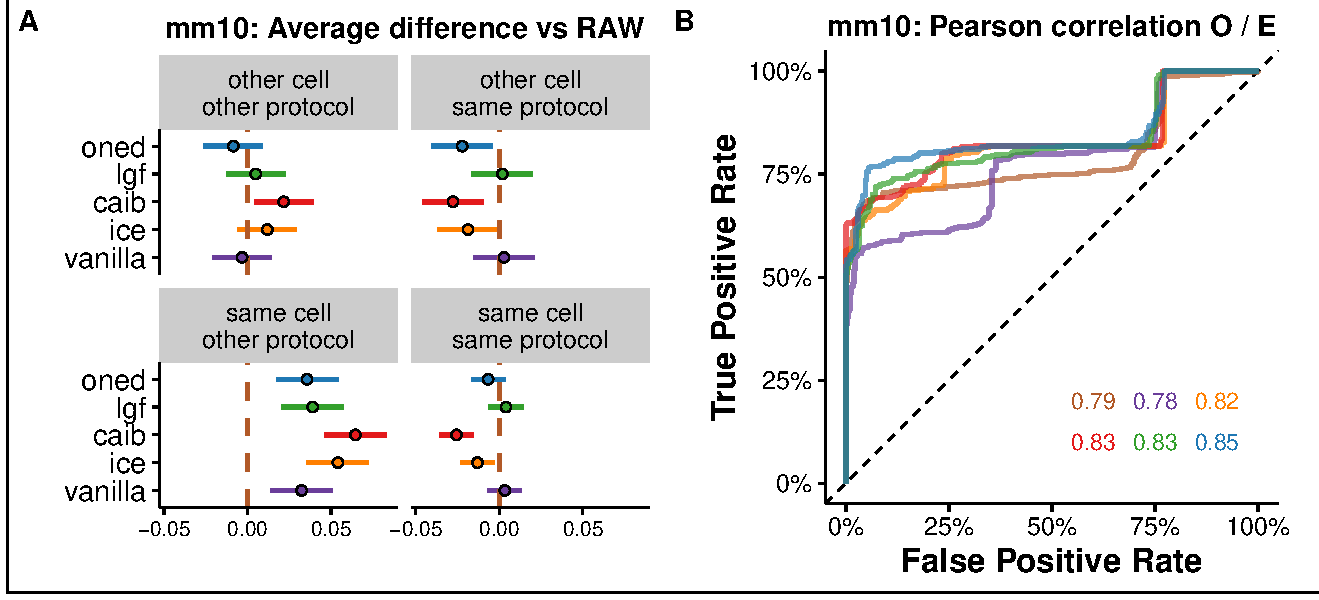
\includegraphics[width=.50\textwidth]
  {img/correlation_normal_figure4.pdf}}
\caption{
Results of the comparison between samples with normal karyotypes. A.
Average changes compared to the raw data on the mouse data set.  B. ROC
curves on the mouse data set. The legend is as in
Figure~\ref{fig:aberrant}.}
\label{fig:normal}
\end{figure}



\subsection{Copy number correction}

Removing the explicit experimental biases enhances the importance of the
copy number in the signal (Figure~\ref{fig:copy_number}). The copy number
is not an experimental bias, but it may be considered an additional source
of bias to be remove. For this reason, \textit{OneD} also allows the user
to correct the copy number and output a euploid-equivalent matrix.

Here, \textit{OneD} segments the linear signal of the total amount of
contacts into piecewise homoegenous regions. This is carried out by a
hidden Markov model whereby the averages of the states are constrained to
be within a discrete factor of each other. This allows the model to detect
regions with a number of copies equal to 1, 2, 3 \textit{etc}. With the
inferred number of copies at hand, \textit{OneD} then normalizes each cell
of the matrix with equation (\ref{eq:cnvnorm}).

Figure~\ref{fig:cnv_correction} shows the effect of this process on the
final Hi-C matrix. Panel \ref{fig:cnv_correction}A indicates that
different normalization methods can either enhance or diminish the signal
in regions with higher copy number. In this example, \textit{ICE}
overcompensates the original bias at the center of the picture and fades
the signal almost entirely. Concomitantly, the signal at the bottom left
of the matrix is enhanced and shows a structure that is not visible in the
raw data. On the contrary, \textit{LGF} strengthen the central region and
the diagonal. \textit{OneD} reduces the level of the central portion by a
factor 2 approximately, but does not otherwise distort the main features
of the region. This example shows that the copy number does not have a
simple and predictable effect on the final matrix. Not taking it into
account may open the door to some normalization artifacts. The result
provided by \textit{OneD} is not necessarily the right one (see
Discussion), but at least it does not correct copy number variations
as a side effect of some other criteria.

\begin{figure}
\centerline{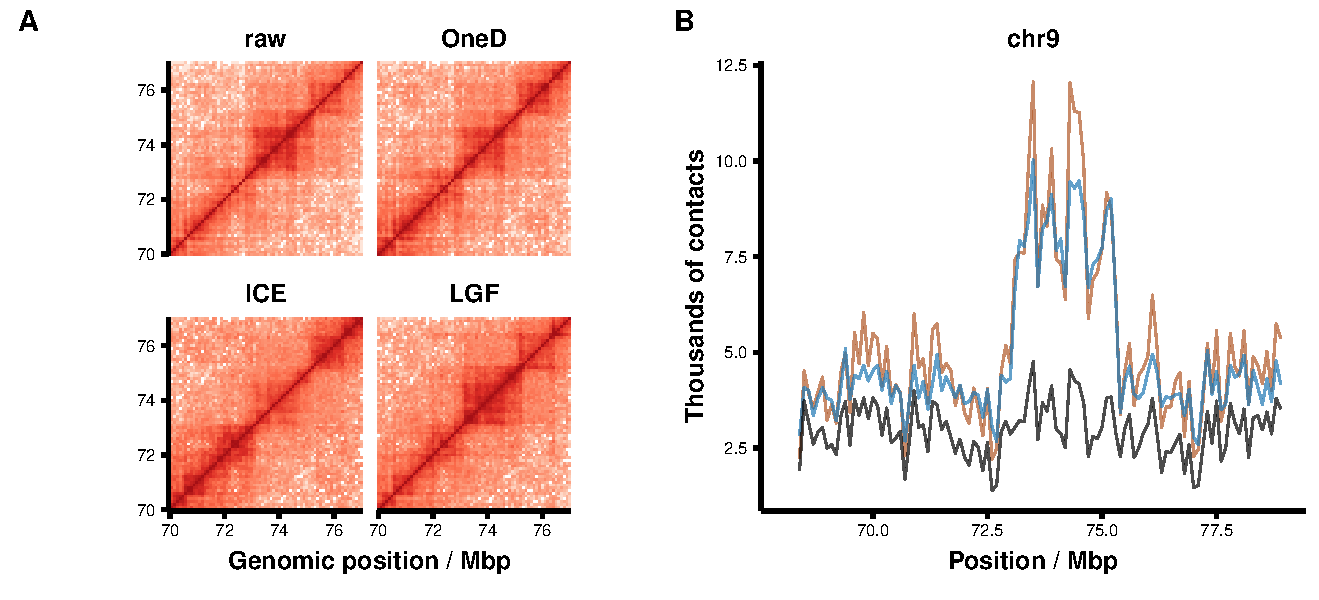
\includegraphics[width=.5\textwidth]
  {img/figure_cnv_correction.pdf}}
\caption{
Copy number correction A. Detail of a Hi-C matrix normalized with
different methods. The central portion has an increased copy number, which
affects normalization. \textit{ICE} fades it away, \textit{LGF} enhances
it and \textit{OneD} reduces the signal by about half. B. Profile of the
total amount of contacts after copy numer correction. The plot shows the
same region as Figure\ref{fig:totals}B. The brown line represents the raw
signal, the blue line represents the signal after bias correction, the
black line represents the signal after bias and copy number correction.}
\label{fig:cnv_correction}
\end{figure}

Figure~\ref{fig:cnv_correction}B shows the total sum of contacts after
correction for the copy number with \textit{OneD}. The signal that
originally showed a sharp transition corresponding to the gain or loss of
a large region, now shows a flat trend throughout the chromosome.

In summary, \textit{OneD} is the only method that can be used to obtain a
euploid-equivalent normalized matrix in cases that the effect of the copy
number must be removed from the signal.



\subsection{Speed}

Finally, we compared the computational speed of the different
normalization methods. One of the main reasons for the broad acceptance of
\textit{vanilla} and \textit{ICE} as standards is the speed of the
available implementation \citep{imakaev2012iterative}. This is even more
significant as current explicit methods \citep{servant2012hitc} are much
slower in comparison.

Unlike the other methods, \textit{OneD} corrects a single variable instead
of the whole matrix, and thus estimates the model parameters much faster
than previous explicit methods. We measured the running time of the
different tools on a 3.3~GHz machine with 62 GB~RAM, always using the
default parameters. Figure~\ref{fig:times}A shows the running times of the
different methods on the samples described in Table~\ref{tab:samples} at
100 kbp resolution. The fastest method is \textit{vanilla} and the slowest
is \textit{LGF}, with an over 100-fold span between the two.

\textit{OneD} is the second fastest method and it always ran in less than
1 min in the conditions of the benchmark. We occasionally encountered
problems where \textit{ICE} ran faster than \textit{OneD} so it is fair to
say that none of them has a definite speed advantage. Throughout this
benchmark, the memory footprint of \textit{OneD} was less than 300 MB.
Interestingly, the running time of \textit{OneD} is much more homogeneous
than that of the other methods. The reason is that the size of the
regression problem to be solved by the \texttt{mgcv} package is always the
same at fixed resolution.

At increasing resolution, the relative rank of the methods remained the
same (Figure~\ref{fig:times}B). The running time of \textit{OneD} remained
close to that of \textit{ICE}. Taken together, these results show that
\textit{OneD} is competitive in terms of computational speed compared to
existing methods.

\begin{figure}
\centerline{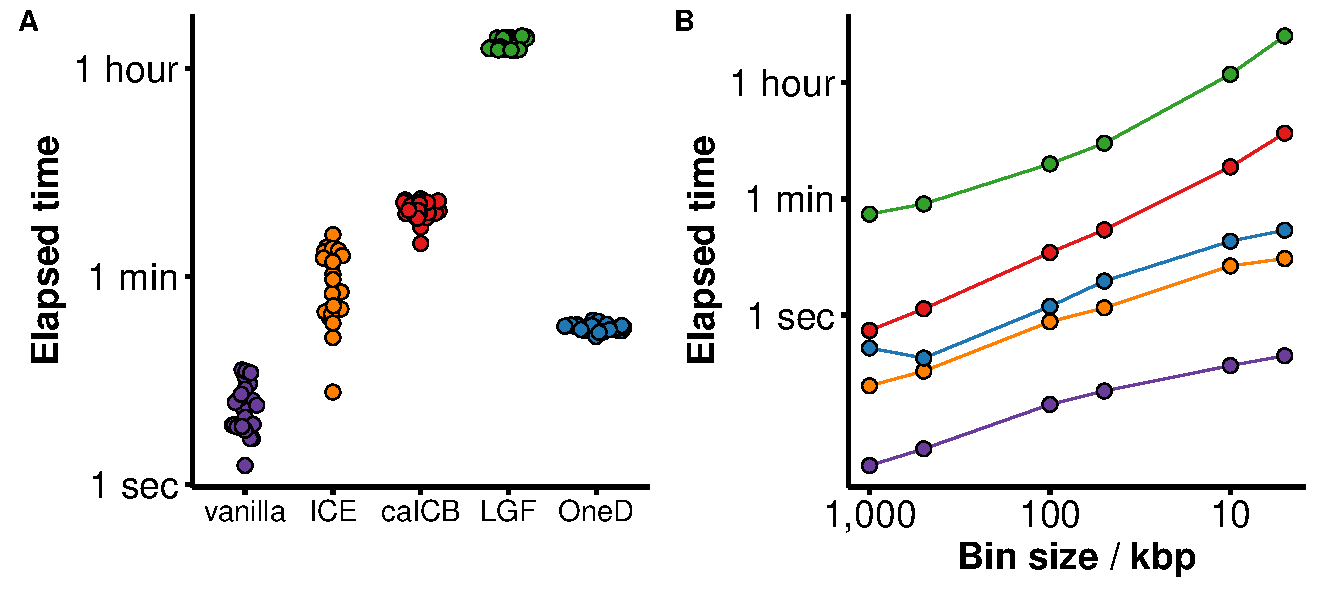
\includegraphics[width=.5\textwidth]
  {img/figure_benchmark_time.pdf}}
\caption{
Computing time of the bias correction methods. A. Total time for the
entire genome at 100 kbp resolution. Each dot corresponds to one sample.
The only method faster than ours under performs in all sample comparisons.
B. Time to correct a reduced genome (chr19-22) of one sample at different
resolutions. Note the logarithmic scale on the y-axis on both panels.}
\label{fig:times}
\end{figure}





%% --------------- Discussion --------------- %%

\section{Discussion and Conclusions}

Here we introduced \textit{OneD}, a fast computational method to normalize
Hi-C matrices. \textit{OneD} was developed ground up to address the need
to normalize data from biological samples with aberrant karyotypes, but it
applies seamlessly to the case of normal karyotypes. We showed that
\textit{OneD} performs significantly better than other methods when the
cells present karyotypic aberrations (Figure~\ref{fig:aberrant}), and that
it performs equally well as the best methods otherwise
(Figure~\ref{fig:normal}). We also showed that \textit{OneD} is
approximately as fast as \textit{ICE}, which makes it competitive from the
point of view of computational speed.

The originality of \textit{OneD} lies in that it projects all the biases
onto a single variable: the total amount of contacts per bin. This allows
greater running speed, while preserving a good performance on samples with
karyotypic aberrations. One of the reasons that \textit{OneD} is better
able to highlight the biological distinctions between samples is that it
only corrects the copy number if specifically requested by the user. The
impact of copy number variations on normalization is rather opaque,
especially if they are treated as implicit biases
(Figure~\ref{fig:cnv_correction}). Treating them as explicit biases with
optional removal seems to be an overall safer strategy.

This raises the question whether variations of the copy number constitute
a biological signal or an artifact. If the biological sample contains
karytoypic aberrations, then its genome is grossly different the reference
so there can be no correct way to normalize the Hi-C signal. The proper
approach would be to use the actual genome of the biological sample as a
reference to construct the contact map. However, this strategy is
presently unfeasible because assembling mammalian genomes is still a hard
problem.

Depending on the intention of the user, the effect of the copy number
should either be kept or removed. This is why \textit{OneD} does not
perform the correction by default, but allows the user to obtain a
euploid-equivalent Hi-C map computed from a hidden Markov model. The
resulting matrices have a near constant amount of contacts per bin, but
the artifacts caused by the mismatch between the genome of the sample and
the reference genome are still present (for instance, the artifacts caused
by large scale inversions are not changed in any way).

Overall, \textit{OneD} constitutes a safe choice to normalize Hi-C
matrices. If the karyotype of the sample is aberrant, it enhances the
biological variation.  If not, it performs at least equally well as other
methods in terms of quality and of computational speed.


\section*{Acknowledgements}

We would like to thank the members of the 4DGenome Synergy project for the
fruitful discussions during project meetings. EV wants to acknowledge
the members of Miguel Beato's laboratory for their insights during lab
meetings.

\section*{Funding}

This work was supported by the Spanish Ministry of Economy and
Competitiveness, ‘Centro de Excelencia Severo Ochoa 2013-2017’,
SEV-2012-0208, ERC Synergy Grant 609989 and...

\vspace*{-12pt}

\bibliographystyle{natbib}
\bibliography{references}

\end{document}
